\section{Sums: The Puzzles and Condition (E)}\label{S-sums}
\subsection{The Two Principles and the Puzzles}
\emph{Principle 1 (number avoidance).} In a sum of numbers and games that are not numbers, a player who can win
can do so without moving in a number~\cite{WinningWays,Siegel2013}.

\emph{Principle 2 (the hottest move).} Move in the component with the highest temperature
(Section~\ref{sec:notation}). For a switch $\game{x}{y}$ between numbers $x>y$, the temperature $(x-y)/2$ is
what each side gains by moving there first, and infinitesimals have temperature $0$. Principle~2 is a
heuristic, not a theorem, but it finds the winning move in every example below.

\begin{figure}[!htbp]
\centering
\begin{subfigure}{0.32\linewidth}\centering
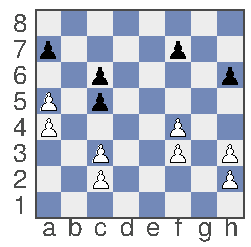
\includegraphics[width=\linewidth]{figures/puzzle71.pdf}
\caption{Puzzle 1}\label{fig:puzzle71}
\end{subfigure}\hfill
\begin{subfigure}{0.32\linewidth}\centering
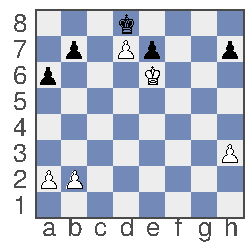
\includegraphics[width=\linewidth]{figures/puzzle72.pdf}
\caption{Puzzle 2}\label{fig:puzzle72}
\end{subfigure}\hfill
\begin{subfigure}{0.32\linewidth}\centering
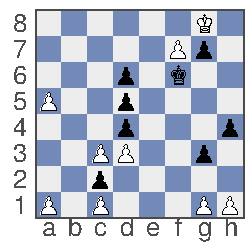
\includegraphics[width=\linewidth]{figures/puzzle73.pdf}
\caption{Puzzle 3}\label{fig:puzzle73}
\end{subfigure}
\caption{Three puzzles of~\cite{Study2025} (cylinder: files a and h adjacent); Table~\ref{tab:puzzles}
gives their exact values. (a)~White wins whoever moves first. (b)~The pawn part is an infinitesimal.
(c)~Puzzle~3 as first drawn: $+\BIG$ (not legal).}
\label{fig:puzzles}
\end{figure}


Table~\ref{tab:puzzles} compares the values first claimed~\cite{Study2025} with the exact ones: the earlier
walk-throughs pick the right winners, but not always the right values.


\emph{Puzzle 1} (Fig.~\ref{fig:puzzle71}) has three components. The earlier values of the c- and f-files are right;
those of files h and a are not. White's a5--a6 still wins
outright, but black, moving first, plays h6$\times$a5 across the seam and leaves $\star$, not a loss, so this
part is $\game{+\BIG}{\star}$, hot, not the number $1$. The total is still a white win whoever moves first, but
play now starts in the h/a component, by far the hottest (Principle~2). White to move plays a5--a6 and wins.
Black to move does best to take on a5 at once, since every other move lets white force a passed pawn (after
h6--h5, a4$\times$h5); white then plays c3--c4 in the next hottest component, and
$1+\star+\game{\game{2}{1}}{0}$ is a white win whoever moves next.

\emph{Puzzle 2} (Fig.~\ref{fig:puzzle72}) has one pawn component, on files h, a and b. The earlier walk-through
finds the right first moves, h3--h4 and a6--a5, and the right outcome, a first-player win. But the value is an
infinitesimal with mean $0$, not $\pm1$, so by Principle~2 it waits until every hot component is settled.
Its king group (Fig.~\ref{fig:kinggroup72}) is not a tr\'ebuchet either. With black to move, the d7 pawn covers
c8 and e8, so Kc7 is forced, and white takes e7 and promotes. With white to move, Kd5, Ke5 and Kf5 all draw:
black wins the d7 pawn, but the white king blockades the e-pawn. The group is a zugzwang for black only, on the
ordinary board \lab{C2} (our solver and the Lichess tablebase) and on the cylinder \lab{C2}, so the real result
of this ten-man position is open.

\emph{Puzzle 3} (Fig.~\ref{fig:puzzle73}) is illegal, with four white pawns on the first rank, and as drawn it
is decided at once, since the pawns on a5 and f7 are passed. On files c and d, white's best move, c3$\times$d4,
leaves $0$. Black's only move, d4$\times$c3, leaves $\game{0}{-1}$: white locks the files with d3--d4, while
black's d5--d4 keeps the spare move d6--d5. Thus $G=\ggame{0}{0\mid -1}=\tinyg{1}$, not $1$, and the legal copy
one rank up, \pos{W c2 c4 d4 / B c3 d5 d6 d7}, has the same value.

\subsection{Condition (E)}
\begin{proposition}[\lab{C1}]\label{prop:condE}
In the pure pawn game, without the passed-pawn rule (play goes on until a side has no move), (E) cannot
be dropped: the sum can be wrong, even in outcome. On the ordinary board with six files and six ranks take
\pos{W a4 f4 / B b4 e5}, where black may take b4$\times$a3 en passant, since white has just played a2--a4. The
whole board is $\game{0}{-4,\,-3\pm2}$, a first-player win, while the sum of its two components is
$\game{-1\star}{-5\star}$, a black win: in the sum the en passant right survives moves in the other component. The two differ
with white to move, as inside larger sums; with black to move, as in the chess position,
both say black wins.
\end{proposition}

\subsection{Two Models}
\emph{Two models.} Our CGT engine computes $S$, as Elkies does~\cite{Elkies1996}, and the independent
whole-board solver $W$. Wherever the two disagree, in every case we tested,
our engine with splitting switched off matches the whole-board solver. The two models agree on every headline value: the $1/8$ and $\upsec\star$
positions of Section~\ref{sec:targets} in all nine settings (Section~\ref{sec:ep}), and the seven-pawn $\nim{2}$
of Section~\ref{sec:star2} in the default setting. Elsewhere they can differ, even in outcome: under the
opponent rule with the e.p.-aware test, \pos{W a3 b3 c2 e2 / B a6 c5 d5 e3} (the first five-file $\nim{2}$ of
Section~\ref{sec:star2-five}) is ${\Uparrow}$ as a sum but $\nim{2}$ on the whole board. Where they differ, we name the model we mean.

\subsection{Two Checks of the Sum Model}\label{S-sumchecks}
Both results of this subsection are computed by one program each \lab{C1}; neither is a proof.

\emph{Sum model against the whole board.} We solved every position without a passed pawn that has at most six
pawns on flat boards three to five files wide, counted up to mirror image and colour swap, in the sum model and on the
whole board ($599{,}098$ positions). We compare only the outcome classes. Table~\ref{tab:censusSW} gives, for each
race rule and passed-pawn test, how often they differ, for all positions, for the hereditarily sum-safe (HSS) ones
and for the others. The default setting is the count rule with the e.p.-aware test.

\begin{table}[!htbp]
\centering
\caption{Positions where the outcome class of the sum model differs from that of the whole board, by passed-pawn
test and race rule: number of differing positions / number of positions.}
\label{tab:censusSW}
\footnotesize
\begin{tabular}{@{}llrrr@{}}
\toprule
test & race rule & all & HSS & not HSS\\
\midrule
textbook & count & $11{,}595$ / $599{,}098$ & $0$ / $539{,}893$ & $11{,}595$ / $59{,}205$\\
textbook & mover & $10{,}496$ / $599{,}098$ & $0$ / $539{,}893$ & $10{,}496$ / $59{,}205$\\
textbook & opponent & $12{,}104$ / $599{,}098$ & $0$ / $539{,}893$ & $12{,}104$ / $59{,}205$\\
e.p.-aware & count & $11{,}300$ / $599{,}098$ & $0$ / $540{,}503$ & $11{,}300$ / $58{,}595$\\
e.p.-aware & mover & $9{,}243$ / $599{,}098$ & $0$ / $540{,}503$ & $9{,}243$ / $58{,}595$\\
e.p.-aware & opponent & $12{,}100$ / $599{,}098$ & $0$ / $540{,}503$ & $12{,}100$ / $58{,}595$\\
\bottomrule
\end{tabular}
\end{table}

\emph{Sum model against real kings.} On the cylinder with eight files and six ranks we fixed the anchors
\pos{Pa3 pa4 Kh4 kb3}, put one component on file d and one on file f with file e empty, and solved the sum with real
kings, queen promotions only, en passant on, and play bounded after the first promotion (the solver's cap~1).
For each side to move the solver returns an upper and a lower bound over W $>$ D $>$ L, from White's point of view; a side is
\emph{exact} if the two agree, and \emph{bounded} otherwise, shown as $[$lower,upper$]$. In
Table~\ref{tab:realkingsum} W, D and L are a win, a draw and a loss for White, and the classes
$\mathcal L$, $\mathcal R$, $\mathcal N$, $\mathcal P$ are the model's, read as white to move, black to move: $\mathcal L$ is
W, W; $\mathcal R$ is L, L; $\mathcal N$ is W, L; $\mathcal P$ is L, W. The anchors alone give exactly this
pattern for $\mathcal P$. The nine P pairs have no passed-pawn component and each contains a locked component of
value $0$, so they test the sum only weakly; the ten N pairs have two live non-passer components of nonzero value.
Of the $38$ sides, $19$ are exact and all agree with the model, and the other $19$ are bounds that contain the model's
result. Every sum of class $\mathcal P$ is bounded on both sides. Bounds confirm nothing beyond that
the model is not contradicted, and all $19$ sums share the same anchors, so the king and anchor placement may matter
at the bound level. One run per position, no independent re-run.

\begin{table}[!htbp]
\centering
\caption{Real-king test of $19$ sums on the cylinder with eight files and six ranks. Components with their values,
the model's outcome class of the sum, and the solver's result with white to move and with black to move.}
\label{tab:realkingsum}
\footnotesize
\setlength{\tabcolsep}{4pt}
\begin{tabular}{@{}lllcll@{}}
\toprule
pair & component on d & component on f & model & white to move & black to move\\
\midrule
P1 & \pos{W d3 / B d4 d5} $(0)$ & \pos{W f2 f4 / B f5} $(1)$ & $\mathcal{L}$ & [D,W] & [D,W]\\
P9 & \pos{W d2 d3 / B d4 d5} $(0)$ & \pos{W f2 f3 / B f4 f5} $(0)$ & $\mathcal{P}$ & [L,D] & [D,W]\\
P21 & \pos{W d2 d4 / B d5} $(1)$ & \pos{W f3 / B f4 f5} $(0)$ & $\mathcal{L}$ & W & W\\
P22 & \pos{W d3 / B d4 d5} $(0)$ & \pos{W f2 / B f4 f5} $(-1/2{\pm}1/2)$ & $\mathcal{N}$ & [D,W] & L\\
P26 & \pos{W d2 d3 / B d4 d5} $(0)$ & \pos{W f2 f3 / B f5} $(1/2{\pm}1/2)$ & $\mathcal{N}$ & W & [L,D]\\
P29 & \pos{W d2 d3 / B d4} $(0)$ & \pos{W f3 / B f4 f5} $(0)$ & $\mathcal{P}$ & [L,D] & [D,W]\\
P35 & \pos{W d2 / B d4 d5} $(-1/2{\pm}1/2)$ & \pos{W f2 f3 / B f4 f5} $(0)$ & $\mathcal{N}$ & [D,W] & L\\
P40 & \pos{W d2 d3 / B d5} $(1/2{\pm}1/2)$ & \pos{W f3 / B f4 f5} $(0)$ & $\mathcal{N}$ & W & [L,D]\\
P48 & \pos{W d2 / B d3 d5} $(-1)$ & \pos{W f2 f3 / B f4} $(0)$ & $\mathcal{R}$ & [L,D] & [L,D]\\
N0 & \pos{W d2 d4 / B d5} $(1)$ & \pos{W f2 / B f3 f5} $(-1)$ & $\mathcal{P}$ & [L,D] & [D,W]\\
N1 & \pos{W d2 d4 / B d5} $(1)$ & \pos{W f2 f3 / B f5} $(1/2{\pm}1/2)$ & $\mathcal{L}$ & W & W\\
N2 & \pos{W d2 d4 / B d5} $(1)$ & \pos{W f2 / B f4 f5} $(-1/2{\pm}1/2)$ & $\mathcal{N}$ & W & [L,D]\\
N3 & \pos{W d2 / B d3 d5} $(-1)$ & \pos{W f2 f3 / B f5} $(1/2{\pm}1/2)$ & $\mathcal{N}$ & [L,W] & [L,D]\\
N4 & \pos{W d2 / B d3 d5} $(-1)$ & \pos{W f2 / B f4 f5} $(-1/2{\pm}1/2)$ & $\mathcal{R}$ & L & L\\
N5 & \pos{W d2 d3 / B d5} $(1/2{\pm}1/2)$ & \pos{W f2 / B f4 f5} $(-1/2{\pm}1/2)$ & $\mathcal{P}$ & [L,D] & [D,W]\\
N6 & \pos{W d2 d3 / B d5} $(1/2{\pm}1/2)$ & \pos{W f2 f3 / B f5} $(1/2{\pm}1/2)$ & $\mathcal{L}$ & W & W\\
N7 & \pos{W d2 / B d4 d5} $(-1/2{\pm}1/2)$ & \pos{W f2 / B f4 f5} $(-1/2{\pm}1/2)$ & $\mathcal{R}$ & L & L\\
N8 & \pos{W d2 d4 / B d5} $(1)$ & \pos{W f2 f4 / B f5} $(1)$ & $\mathcal{L}$ & W & W\\
N9 & \pos{W d2 / B d3 d5} $(-1)$ & \pos{W f2 / B f3 f5} $(-1)$ & $\mathcal{R}$ & L & L\\
\bottomrule
\end{tabular}
\end{table}
